\chapter{Úvod}

V době vysokorychlostního a stabilního internetu je využívání vzdálených uložišť běžnou záležitostí. Pro většinu uživatelů je to nástroj
pro jednoduchou synchronizaci dat napříč několika zařízeními od mobilního telefonu po stolní počítač. Pokud vezmeme v úvahu pouze velká datová centra,
jedná se pravděpodobně o nejlevnější a nejspolehlivější způsob uchování dat, protože tyto centra mají velkou kapacitu úložného prostoru a také zálohy na
softwarové i hardwarové úrovni. Pod pojmem vzdálené uložiště si nemusíme představit jen velká datová centra se stovkami serverů, může se jednat o relativně malé uložiště
ve firmě nebo dokonce o osobní/domácí řešení. Pro využívaní osobních/firemních uložišť se lidé uchylují v případech, je-li třeba uložit osobní nebo
určitým způsobem citlivá data, která by nemohla být poskytnuta třetí straně. Nabízená řešení také nemusí poskytovat potřebnou funkcionalitu nebo jejich finanční model
nesplňuje zákazníkova kritéria.

V průběhu let byly vyvinuty protokoly řešící sdílení souborů jako FTP, NFS a mnohé další. Sdílení souborů je komplexní záležitostí a obsahuje
velké množství parametrů. Každý protokol se zaměřuje jen na určité parametry jako zabezpečení a spolehlivost přenosu, oprávnění pro jednotlivé
uživatele a soubory, synchronizace modifikovaných souborů apod nebo pojme daný parametr odlišným způsobem. V dnešní době je většina komerčně využívaných
aplikací vystavěna na proprietárních protokolech nebo na protokolech umožňující obecnější použití. Jedním z nejpoužívanějších aplikačních protokolů
bude Hypertext Transfer Protokol neboli HTTP.

Cílem této práce je prozkoumat aktuální nabídku a možnosti na poli vzdálených uložišť a navrhnout aplikaci pro řízený přístup ke vzdáleným dokumentům pro
platformu \mbox{GNU/Linux}. Aplikace bude zaměřena na řízený životní cyklus souborů s vynucenými oprávněními pro jednotlivé soubory daná vzdáleným uložištěm.
Komunikace skrze HTTP protokol byla definovaná externím zadavatelem. Zdrojové kódy jsou dostupné na veřejném Github repozitáři.
\footnote{\url{https://github.com/PlayerBerny12/VUT-IBT-Code}}

\chapter{Motivace a existující řešení}

Popularita a využití vzdálených uložišť roste, protože lidé využívají více zařízení a potřebují mezi nimi jednoduchou synchronizaci nebo na jednom souboru
potřebuje spolupracovat více lidí. Dalším podnětem využívání vzdálených uložišť je většího množství dat a potřeba tyto data efektivně sdílet a bezpečně uložit.
Postupně se digitalizují další systémy například ve státní správě nebo dalších podnikatelských sektorech. 

Na trhu je velké množství služeb zaměřujících se na různé klientské potřeby. Diverzita nabídky je až překvapivě velká. Většina se zaměřuje na ukládání a sdílení
dat ve svém ekosystému, které jsou určené pro široké použití. Pokud jsou požadavky specifické, tak možnost vlastní konfigurace není možná. Pro částečnou úpravu 
nebo automatizaci procesů lze využít poskytované API, ve většině případu se jedná o variantu REST API. Poslední možností je vystavění obdobné služby z několika
existujících aplikací nebo vytvoření nové.\\

\noindent V kontextu této práce jsou požadavky následující: 

\begin{itemize}
    \item Dodržování oprávnění i na klientském systému
    \begin{itemize}
        \item read-only
        \item write-only
        \item read/write
    \end{itemize}
    \item Životní cyklus souboru (stažení)
    \begin{itemize}
        \item stažení
        \item případná modifikace
        \item smazání souboru po vypršení platnosti
    \end{itemize}
    \item Autentifikace
    \begin{itemize}
        \item uživatelské jméno a klientský certifikát
        \item uživatelské jméno a heslo
    \end{itemize}
\end{itemize}

\section{Současná řešení}

Pro bližší analýzu byl vybrán vzorek služeb a programů obsahující velké ekosystémy služeb po open source aplikace. Zkoumáno bylo několik parametrů,
jako poskytovaná funkcionalita pro jednotlivce a firmy, cena, integrace s ostatními systémy a aplikacemi apod. Obecně nelze jednoznačně určit nejlepší uložiště, 
ale je možné poukázat na rozdílné vlastnosti a vyzdvihnout kladné. Koncový uživatel se následně může rozhodnout dle svých potřeb.

\section{Google Drive}

Pro synchronizaci obsahu z Google Drive na osobní počítač se využívá aplikace pojmenovaná Google File Stream. Je možné ji provozovat pouze na systémech
Windows a Mac OS.\cite{GoogleFileStream} Pro Linuxové distribuce lze využít například neoficiální open source aplikaci 
Google Drive OCamlFUSE\footnote{\url{https://github.com/astrada/google-drive-ocamlfuse}} využívající technologii
FUSE, která bude popsána v následující kapitole \ref{sec:fuse}. Google Disk poskytuje plně funkční webové rozhraní,
ve kterém je možné dokumenty přímo upravovat bez nutnosti stahování. Problém nenastal ani v případě konkurenčních Microsoft Office dokumentů. 

Google Workspace (dříve Google Suite) je možné pořídit v několika balíčcích. Například balíček Bussiness Standard nabízí 2 TB uložiště za 10,40 EUR měsíčně.
Balíček obsahuje další služby jako firemní email a schůzky až o 150 účastnících na Google Meet.\cite{GoogleWorkspace}

Každý uživatel má vlastní disk s omezenou kapacitou podle balíčku. Na disku lze vytvářet standartní složkovou hierarchii a je možné sdílet jednotlivé soubory nebo
obsah složek s ostatními Google uživateli. Verze Enterprise umožňuje vytváření dalších disků, na které je možné přiřadit seznam uživatelů. Každý uživatel
má nastavenou jednu z 6 rolí, které vymezují jeho možnosti. K dispozici je API, která pokrývá veškeré možnosti webového rozhraní jako vytvoření souboru,
sdílení atd.\cite{GoogleAPIReference}

\section{Dropbox}

Dropbox má oficiální balíčky své aplikace pro Ubuntu a Fedoru, případně je možné si aplikaci zkompilovat ze zdrojových souborů. Podpora Windows a Mac OS je samozřejmostí.
Z práce „Personal Cloud Storage Benchmarks and Comparison“ lze vyčíst, že Dropbox se zaměřuje na efektivitu přenosu a minimální zatížení sítě.
Využívá menší množství TCP spojení oproti jeho konkurentům a také stejně jako Google Drive komprimuje data před odesláním.\cite{CloudStorageComparison}
Toto řešení nemusí dosahovat nejvyšší výkonosti, ale nezatěžuje tolik infrastrukturu. 

Webové rozhraní je více orientováno na správu souborů a jejich historii. Nabízí jednoduché obnovení smazaných souborů nebo návrat k předchozí verzi.
Nenabízí tolik možností jako Google Drive, ale upravovat dokumenty ve webovém prohlížeči lze také. Na výběr je mezi Microsoft Office Online nebo Google Worksapce.
Sdílení souborů a složek je možné i s uživateli, kteří nemají Dropbox účet.

Balíček Plus za 9,99 EUR měsíčně dává uživateli přístup ke 2 TB uložišti. Firemní balíčky obsahují rozšíření pro lepší správu uživatelů, vytváření skupin
a admin panel/konzole. Dropbox má také API nabízející dostatečnou funkcionalitu pro případnou integraci s jinými systémy apod.\cite{Dropbox}

\section{pCloud}

Poskytovatel pCloud podporuje nejpoužívanější platformy, a to včetně mobilních. Za 9,99 EUR měsíčně dostane uživatel 2 TB uložiště. Jako jediný z poskytovatelů
v analýze nabízí balíček s jednorázovou platbou za cenu 350 EUR. Jedná se o identický balíček, pouze forma platby se liší. Všechna data jsou přenášena přes
šifrovaný kanál a všechny kopie souborů na pěti různých serverech jsou šifrovaná 256bitovým AES klíčem.\cite{pCloud}

Webové rozhraní je jednoduché, avšak oproti konkurentům má méně funkcí. Lze zobrazit náhled dokumentů, ale upravovat je nelze. Každý soubor má tzv. revize 
a je možné obnovit obsah souboru na vybranou revizi. Revize jsou uchovány po dobu jednoho roku. Soubory je možné sdílet i s uživateli, kteří nemají účet u pCloudu. 

Pro firemní zákazníky je nabízený rozšířený management uživatelů a monitoring s logy aktivity jednotlivých uživatelů.

\section{Syncthing}

Open source aplikace Syncthing synchronizuje soubory peer-to-peer. Nejedná se o čistou peer-to-peer architekturu, protože jeden z uzlů může být
nastaven jako server a veškeré data budou synchronizována vůči tomuto uzlu. Syncthing je možné provozovat na většině dnešních systémů jako Windows, Linux, BSD a
Mac OS.\cite{Syncthing}

Aplikace poskytuje webové rozhraní, které je určené pouze pro nastavení parametrů jako discovery protokol pro objevování ostatních uzlů, jaké složky mají být synchronizovány
nebo kolik verzí jednotlivých souborů má být uchováváno a mnoho dalšího. Velká přizpůsobivost umožňuje upravit fungování aplikace vlastním potřebám, na druhou
stranu bude náročné udržovat systém s větším množstvím uživatelů vystavěný na této aplikaci. Jedná se tedy spíše o domácí řešení.

\section{Shrnutí}

Trendy na poli vzdálených uložišť určují velké firmy jako Google nebo Micorsoft. Apliakce One Drive od Microsoftu nebyla blíže analyzovaná, protože se jedná
o službu pouze pro platformu Windows. Důkazem tohoto jevu je například integrace aplikací obou těchto firem do webového rozhraní Dropboxu.

Všichny služby mají webové rozhraní, ke kterému je aplikace synchronizující obsah uložiště občas braná jako doplňek. Sdílení nebo obnova předchozí verze souboru
je vždy možná ve webové aplikaci, ale ne vdžy jsou tyto akce dostupné v desktopové aplikaci.

Aplikace na jejíž základě je vytvořená tato práce nebude klasickou synchronizační apliakcí. Bude se pracovat jen s jednotlivými soubory, na kterých bude uživatel chtít
pracovat (zobrazit nebo upravit obsah). Nebude možné synchronizovat celé uložiště, ale vždy jen jeden specifický soubor. Jedná se tedy spíše o náhradu možnosti upravovat
soubor přímo ve webovém prohlížeči jako to umožňuje například Google Drive.

\chapter{Návrh řešení a použité technologie}

Prvním krokem navrhovací fáze bylo seznámení se zadáním a požadavky. Externí zadavatel dodal podrobnou dokumentaci REST API pro validované datové uložiště, která
byla stěžejním dokumentem při návrhu. API obsahuje funkce pro ověření spojení, autentifikaci a práci se soubory. VDU nebylo při vzniku této práce k dispozic a proto
byl pro potřeby vývoje vytvořen mock server na základě API dokumentace.

Pro vynucení práv jednotlivých souboru je standartní souborový systém nevyhovující, protože po stažení souboru do počítače uživatele se ztrácí veškerá kontrola nad
tímto souborem. Po konzultaci s vedoucím práce, dokterem Markem Rychlým, byla zvolena technologie FUSE neboli Filesystem in userspace. FUSE umožňuje vytvořit virtuální
souborový systém a implementovat jednotlivé operace jako čtení, zápis atd.

\section{Případy užití}

Diagram případu užití zachycuje celý systém jako celek sestavený z jednotlivách funkcí a jejich návazností, které je třeba dále analyzovat a specifikovat v dalších
fázích návrhu.

\begin{figure*}[h]
    \centering    
    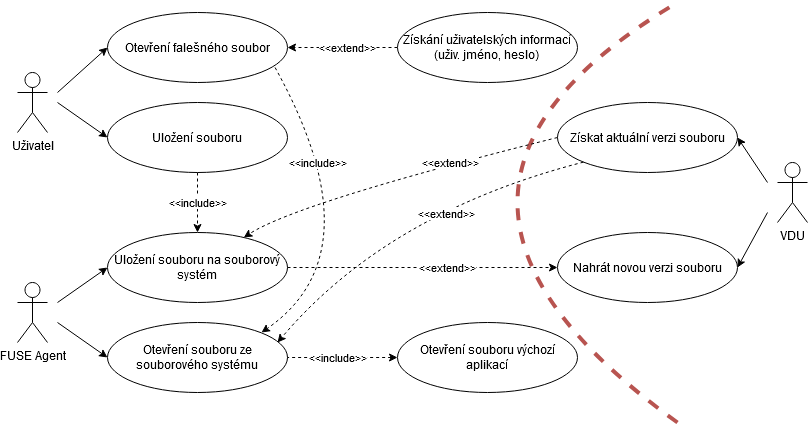
\includegraphics[width=1\linewidth]{other-fig/use_case_diagram.png}
    \caption{Diagram případu užití}
    \label{fig:use_case}
\end{figure*}

Na diagramu \ref{fig:use_case} vystupují tři aktéři a to uživatel, FUSE agent/démon a VDU. Implementace VDU není obsahem této práce, proto je oddělena červenou
přerušovanou čarou. V diagramu není zanesená například autentifikace, na které závisí veškerá Komunikace s VDU. Diagram by byl poté nepřehledný, proto byla tato
část vypuštěna.

Všechny akce jsou spouštěny přímo uživatelem, některé vyvolají spuštění funkce FUSE démona. Jedná se například o uložení, otevření nebo přejmenování souboru ve virtuálním
souborovém systému. Speciální případ nastávám při otevření url s vlastním protokolem, který má spustit aplikaci, jež je k danému protokolu v systému přiřazena.
Na tuto URL bude uživatel přesměrován z webového rozhraní VDU. Příkladem protokolu spouštějící aplikaci v systému může být \texttt{mailto}, využívaný často u webových aplikací.
Přesměrování na adresu s tímto protokolem otevře správce elektronické pošty. 

K námi definovanému protokolu pojmenovaném „\texttt{vdu}“ je třeba mít v systému přiřazenou aplikaci. Na základě přístupového tokenu uloženého v URL 
(\texttt{vdu://<přístupový token>}) se spustí daná aplikace, která stáhne žádaný soubor z VDU na virtuální souborový systém. Na základě této znalosti byly
uskutečněné zásadní rozhodnutí při návrhu architektury.
 
\section{Architektura}

Zvažovány byly dvě implementační varianty, jedna verze pracoval pouze s jednou aplikací a to byl FUSE démon. Druhá vraianta rozdělila funkčnost do dvou aplikací, jednou 
z nichž byl FUSE démon a druhou byla klasická apliakce napsaná například v C++. V tomoto případě by samostatná aplikace obsluhovala komunikaci s VDU a byla by spouštěna
na základě volání FUSE démona nebo uživatele.

První variantu by šlo zpracovat dvěma podobnými způsoby vedoucí ke stejnému řešení. FUSE démon je napsaný v jazyce C, takže první zvažovaná varianta byla implementace
celá apliakce jednom jazyce. Druhou možností by bylo vytvoření C++ knihovny, která by měla interface pro jazyk C, aby mohl vytvořenou knihovnu využít FUSE démon. Nejedná se
však o nijak kriticky náročnou aplikaci na výkon, takže by byla varianta s C++ knihovnou upřednostňována.

Se znalostí z diagramu případu užití, že je třeba mít registrovanou apliakci, která bude spuštěna po otevření speciální URL. I kdybychom vzali v úvahu místo URL soubor
se speciální koncovkou (např. *.vdu) obsahující přístupový token, který by si uživatel stáhnul z VDU, tak k otevření tohoto souboru je třeba mít také přiřazenou aplikaci, která
by danou akci obsloužila. Démon běžící na pozadí po celou dobu běhu systému, nemůže být přiřazen jako obsluhující aplikace otevření speciální URL. Na základě těchto okolností
byla vybrána varianta se dvěma aplikacemi.

\begin{figure*}[h]
    \centering
    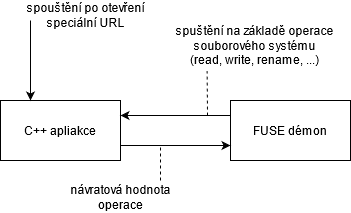
\includegraphics[width=0.47\linewidth]{other-fig/architecture.png}
    \caption{Architektura}
\end{figure*}

Pokud FUSE démon má vykonat akci, pro kterou nemá dostatečné informace, spustí jako další subproces druhou hlavní aplikaci a počká na návratovou hodnotu, na základě
které se rozhodne, jakým způsobem onu akci dokončí. Může se jednat o případy jako jestli je soubor určený jen pro četní nebo i zápis, nebo jestli daný soubor už není
validní, protože vypršel datum expirace apod.

V této variantě je FUSE démon velmi minimalistický a zybtek funkcionality je implementován do druhé aplikace, která je spouštěna jen na vyžádání, narozdíl od neustále
běžícího démona. Démon tedy po celou dobu běhu zabírá méně místa, protože nemusí mít načtená v paměti všechny potřebné knihovny. Na druhou stranu potřené knihovny mohou 
být v paměti namapované, protože jsou využíváné jinými aplikacemi. Démon musí být spuštěný s právy superuživatele \texttt{root} a menší množství kódu spuštěného s vysokými
oprávněními implikuje menší náchylnost na bezpečnostní chyby. Démon bude totiž pouštět druhou aplikaci s oprávněními přihlášeného uživatele.

\subsection{Diagram tříd}

Aby implementace byla co nejjednodušší a nebylo třeba již uvažovat nad dalšími rozhodnutími, byl vytvořen diagram tříd \ref{fig:class_diagram_design}, který relativně
podrobně vizualizuje jaké třídy s atributy a metodami je třebe implementovat. Jedná se pouze o návrh, který se v průběhu vývoje bude dynamicky měnit. Pokud je návrh
kvalitní a programátoři se ho sanží dodržet, neměl by být výsledek zásadně rozdílný.

\begin{figure*}[h]
    \centering
    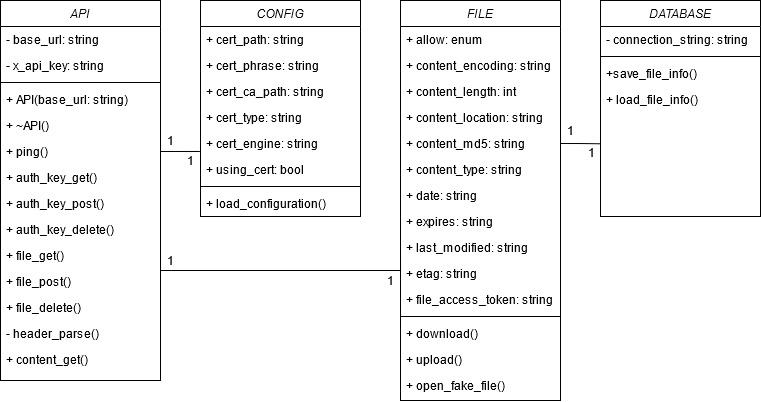
\includegraphics[width=1\linewidth]{other-fig/class_diagram_design.png}
    \caption{Diagram tříd - návrh}
    \label{fig:class_diagram_design}
\end{figure*}

Na obrázku \ref{fig:class_diagram_implementation} je možné vidět diagram tříd naimplementovaného programu. Na první pohled vypadá velmi rozdílně, po bližším prozkoumáním
lze vidět jednu novou třídu oproti návrhu. Jedná se třídu zobrazující notifikace pro uživatele, takže nemá vliv na hlavní funkcionalitu.

\begin{figure}
    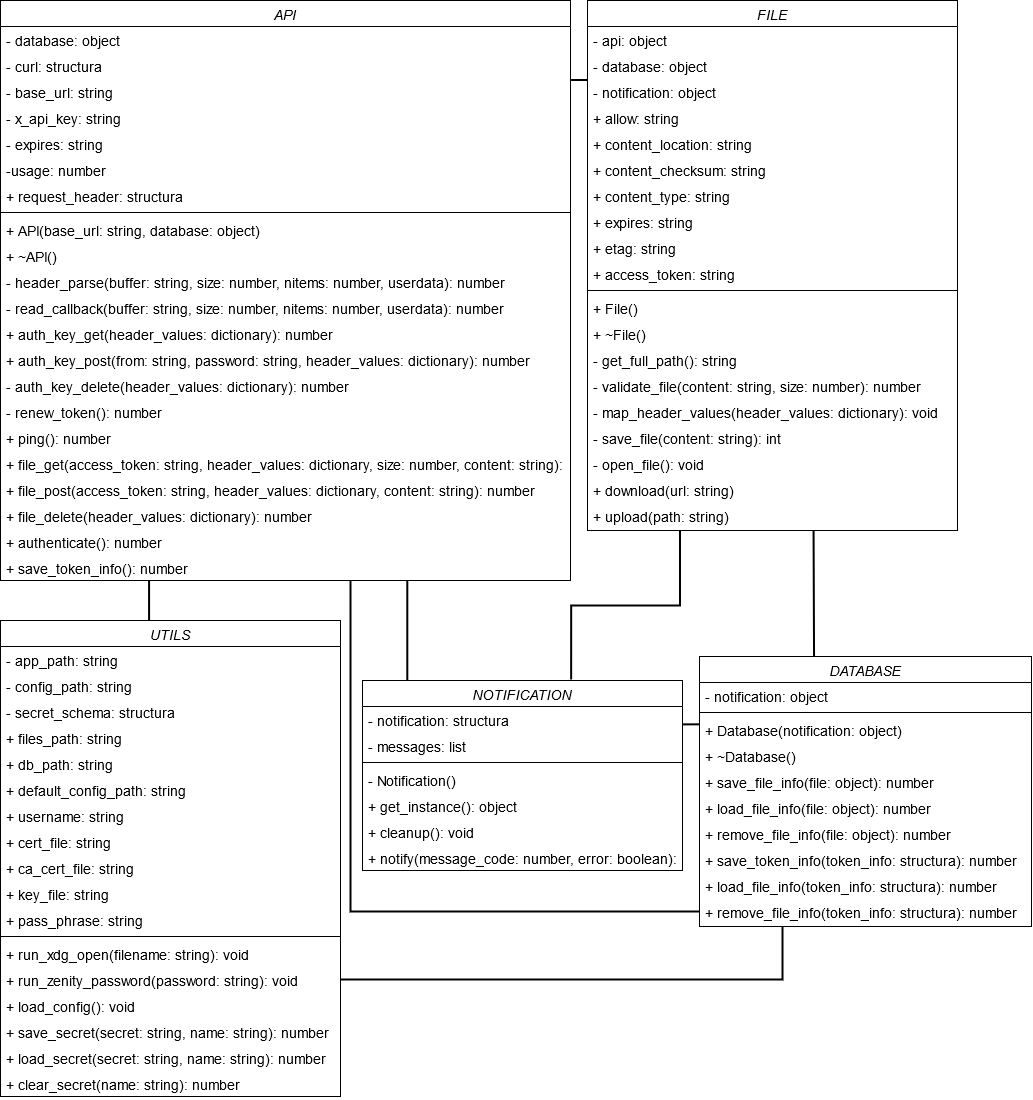
\includegraphics[width=1\linewidth]{other-fig/class_diagram_after_implementation.png}
    \caption{Diagram tříd - implementace}
    \label{fig:class_diagram_implementation}
\end{figure}

\section{Technologie}
\subsection{GNU/Linux}
\subsection{C++/C}
\subsection{OpenAPI}
\subsection{HTTP}

\cite{RFC7231}
\cite{HTTP3}

\subsection{Mock server}

\cite{MockServer}

\subsection{Souborový systém v uživatelském prostoru (FUSE)}
\label{sec:fuse}

\cite{FuseOrNotToFuse}
\cite{HardeningFUSE}

\subsection{DBus}
\subsection{Keyring}

\cite{Keyring}

\chapter{Popis implementace a nasazení aplikace}

- Seznam použitých knihoven

\section{Definice API}
\section{Mock server}
\section{Vyžívané cesty/soubory v Linuxové adresářové struktuře}
\subsection{Konfigurační soubor}
\subsection{SQLite databáze}
\section{Autentifikace}
\section{Práce se soubory}
\subsection{Otevření souboru v příslušné aplikaci}

\cite{xdg}

\section{Nasazení aplikace}
\subsection{DPKG} %APT
\subsection{RPM} %DNF/YUM
\subsection{Sestavení ze zdrojových souborů}

\chapter{Testovací sada}

- Testy pro funkce třídy API

\section{Google Test}

\chapter{Závěr}



